\documentclass[11pt,a4paper]{report}
\usepackage{graphicx}
\usepackage{amsmath}
\usepackage{fancyhdr}
\usepackage{cite}
\usepackage{framed}
\usepackage{a4wide}
\usepackage{float}
\usepackage{epsfig}
\usepackage{longtable}
\usepackage{enumerate}
\usepackage{afterpage}
\usepackage{multirow}
\usepackage{ragged2e}
\usepackage{gensymb}
\usepackage{amsfonts} 
\usepackage[left=3.5cm,top=3cm,right=3cm,bottom=2.5cm]{geometry}
\usepackage{setspace}           
\usepackage{float}
\usepackage{txfonts}
\usepackage{lipsum}

\newcommand{\Usefont}[1]{\fontfamily{#1}\selectfont}

\usepackage{lscape} % for landscape tables
\renewcommand{\baselinestretch}{1.7} 

\usepackage{blindtext}
\usepackage{xpatch}
\usepackage{url}
\usepackage{leqno}
\usepackage{subcaption}

\linespread{1.5}
\usepackage[intoc, english]{nomencl}
\hyphenpenalty=5000
\tolerance=1000
\usepackage[nottoc]{tocbibind}
\bibliographystyle{IEEEtran}
\renewcommand{\bibname}{References}

%*******************************************************************
%                        Header and Footer   
% This is not required in Technical reports submitted to CET ECE department.
% Please leave it commented                       
%*******************************************************************
\pagestyle{fancy}
\fancyhead{}
%header and footer section
\renewcommand\headrulewidth{0.1pt}
\fancyhead[L]{\small\centering }
\fancyhead[R]{}
\renewcommand\headrulewidth{0.1pt}
\fancyfoot[R]{\small GEC Thiruvanathapuram}
\renewcommand\footrulewidth{0.1pt}
\fancyfoot[C]{\footnotesize \thepage}
\fancyfoot[L]{\small Department of CSE}
%*******************************************************************


%*********************Figures*****************************
% Save all figures in the folder figures and include them in your 
% report using the command \includegraphics{figure-name}

\graphicspath{{figures/}}

% figure files can be in jpeg,jpg, png or pdf formats
%*******************************************************************


\begin{document}
	
	
%****The entries in this section are to be filled in by the student with appropriate values *************

% These values are used thoroughout the report 
% please fill in the appropriate values

\gdef \title{Intelligent Incident Surveillance Response System} % Seminar title
\gdef \author{Ashna Joy}	 %student name
\gdef \dept{Computer Science \& Engineering} %Department
\gdef \degree{Bachelor of Technology} %degree
\gdef \branch{Computer Science \& Engineering} %branch
\gdef \college{Government Engineering College}
\gdef \collegeplace{Thiruvananthapuram}
\gdef \rollno{TVE22CS-P012} %KTU Reg No
\gdef \deptabbr{Dept.of CSE} %Dept name abbreviation

\gdef \guide{Prof.George Thomas}%Seminar guide
\gdef \guidedes{Assistant Professor }%Seminar guide designation

\gdef\semcordinatorA{Prof.George Thomas  }% Seminar coordinator 1 
\gdef \semcordinatorAdes{Assistant Professor }% Seminar coordinator 1 designation

\gdef \semcordinatorB{Prof.Anjali Devi A J. } % Seminar coordinator 2 
\gdef \semcordinatorBdes{Assistant Professor }% Seminar coordinator 2 designation

\gdef \hod{Dr.Jayasree P K} %Head of Department
\gdef \hoddes{Professor and Head} %HOD designation

\gdef \acadyear{2022 - 2026} % Academic year
\gdef \month{November  2025} %Month of Report submission
\gdef \date{23-10-2025} %Date of signing the declaration

%*******************************************************************
% The font pages. The source tex files are there in the folder
%==================================coverpage.tex================================


\newenvironment{coverpage}
\thispagestyle{empty}
\begin{titlepage}
	\begin{center}
		{\Usefont{phv} \Large \bf \title \par}
		\vspace*{20pt}
		\large \em \Usefont{pzc}{ 
			A Project Report \par
			Submitted to the APJ Abdul Kalam Technological University\\
			in partial fulfillment of requirements for the award of degree}\\ [.15\baselineskip] \par
   
            \vspace*{20pt}
            
		\Usefont{ppl} {\bfseries  \degree}\\
		in\\
		{\Usefont{ppl} {\bfseries \branch}}\\
		by\\[10pt]
		\bf {\author}\\[5pt]
		\bf{\rollno}
		\vspace*{20pt}
		\centering
		\begin{figure}[h!]
			\centerline{
\includegraphics[scale=0.65]{cet_logo_1.jpeg}}
		\end{figure}
  
		\vspace{10pt}
		\footnotesize{\bf Computer Science \&  Engineering} \par
		\bf{GOVERNMENT ENGINEERING COLLEGE} \par
		\bf{Thiruvananthapuram}\\
  \bf{\month}
		
	\end{center}		
\end{titlepage}	
 %Unless essential Do not edit this tex file



%%********************Certificate*******************

% To print name of only the seminar coordinator 1 in the certificate page
%%==================================certificate1.tex================================
% To print name of only the seminar coordinator 1 in the certificate page

\newenvironment{certificate1}

	\newpage
	\begin{center}	
		%\vspace{1.5cm}
		
		\textbf{DEPARTMENT OF ELECTRICAL \& ELECTRONICS ENGINEERING}	
		\textbf{GOVERNMENT ENGINEERING COLLEGE, BARTON HILL}  
		\textbf{THIRUVANANTHAPURAM}
		
		\textbf{\acadyear} 
	\end{center}
	\vspace{30pt}
	\begin{center}
		\includegraphics[scale=0.6]{gecbh.jpg}	
	\end{center}
 \vspace{20pt}
	\begin{center}
		\textbf{CERTIFICATE}
	\end{center}
	\vspace{10pt}
	This is to certify that the report entitled \textbf{\title} submitted by \textbf{\author}\hspace*{2pt}(\rollno), to the APJ Abdul Kalam Technological University in partial fulfillment of the B.Tech.\ degree in \branch \hspace*{2pt} is a bona fide record of the seminar work carried out by him under our guidance and supervision. This report in any form has not been submitted to any other University or Institute for any purpose.
	
	
	\begin{singlespace}
		\vspace*{2cm}
		\begin{table}[h!]
			\centering
			\begin{tabular}{p{7cm} p{0.9cm} p{7cm}} 
				\textbf{\guide} && \textbf{\hod} \\
				(Seminar Guide and Coordinator) &&  (Professor and Head)\\
				\guidedes & & \hoddes\\ 
				Dept.of EEE && Dept.of EEE\\ 
				&& \\
                && \\
				&& \\
			\end{tabular}
			
		\end{table}
		
		
	\end{singlespace}
	
	\thispagestyle{empty}



 

% To print names of both the seminar coordinators in the certificate page
%==================================certificate2.tex================================
% To print names of both the seminar coordinators in the certificate page
\newenvironment{certificate2}

\newpage
\begin{center}	
	%\vspace{1.5cm}
	
	\textbf{DEPARTMENT OF COMPUTER SCIENCE \& ENGINEERING}	\\
     \textbf{Government Engineering College}	
	\textbf{Thiruvananthapuram}\\
	\textbf{\acadyear} 
\end{center}

\begin{center}
	
\includegraphics[scale=0.6]{cet_logo_1.jpeg}
\end{center}
\begin{center}
	\textbf{CERTIFICATE}
\end{center}

This is to certify that the report entitled \textbf{\title} submitted by \textbf{\author} \hspace*{2pt}(\rollno), to the APJ Abdul Kalam Technological University in partial fulfillment of the B.Tech.\ degree in \branch \hspace*{2pt} is a bona fide record of the project work carried out by her under our guidance and supervision. This report in any form has not been submitted to any other University or Institute for any purpose.


\begin{singlespace}
	\vspace*{1cm}
	\begin{table}[h!]
		\centering
		\begin{tabular}{p{7cm} p{0.9cm} p{7cm}} 
			\textbf{\semcoordinatorA}&&\ \textbf{External Auditor}\\
			(Project Guide \& Coordinator)\\
			\semcoordinatorAdes \\ 
			\deptabbr \\
		\end{tabular}
		
	\end{table}
	
	\vspace*{1.3cm}
	\begin{center}
		\begin{tabular}{p{7cm} p{0.9cm} p{7cm}}
			%\hline
		\end{tabular}
	\end{center}
\end{singlespace}

\thispagestyle{empty}




 %uncomment this and comment the previous line

%%***************************************************


%==================================declaration.tex================================
%
\newpage
\newenvironment{declaration}
\thispagestyle{empty}
\begin{center}
\vspace*{50pt}
\textbf{DECLARATION}\\
\end{center}
I, \author, hereby declare that the project report entitled {\bf{\title}}, submitted in partial fulfillment of the requirements for the award of the degree of Bachelor of Technology of APJ Abdul Kalam Technological University, Kerala, is a bona fide record of work carried out by me under the supervision of \guide.\par
This submission represents my original work. Wherever the ideas or words of others have been included, they have been properly and accurately acknowledged through citation and reference.\par
I further declare that I have adhered to the principles of academic honesty and integrity and have not misrepresented, fabricated, or falsified any data, fact, or source in this submission. I understand that any violation of the above will invite disciplinary action by the institute and/or the University. This report has not previously formed the basis for the award of any degree, diploma, or similar title of any other university or institution.

\noindent \begin{minipage}{0.45\linewidth}
\vspace{2.5cm}
\begin{flushleft}
\begin{flushleft}
Trivandrum\\
\date
\end{flushleft}
\vspace{2.5cm}


\end{flushleft} 
\end{minipage}
\hfill
\begin{minipage}{0.45\linewidth}
\begin{flushright}                                      
\vspace{1cm}

\author\\


\end{flushright} 
\end{minipage}
\thispagestyle{empty}
 %Unless essential Do not edit this tex file

\pagenumbering{roman} 

%%********************************Abstract***********************
%============================= abstract.tex================================
\vspace*{50pt}




\begin{center}
\textbf{ABSTRACT}\\
\end{center}
%\addcontentsline{toc}{chapter}{\numberline{}Abstract}%
\addcontentsline{toc}{chapter}{Abstract}%
\newenvironment{Abstract}
\vspace{20pt}
The proposed project aims to design and implement a smart vehicle surveillance system that enhances the security of a car by integrating a surveillance feature capable of recording video footage and sending real-time alerts based on various event triggers. The system leverages the existing cameras in a car, such as surround view cameras, to provide comprehensive video coverage from all angles around the vehicle. When an event occurs, such as honking, sudden braking, alarm activation, suspicious person detection, or break-ins, the system automatically records video footage. The footage is then uploaded to a cloud-based server, allowing car owners to view it remotely.\par
The system also sends real-time notifications to the car owner, providing options to view the footage. This enables car owners to stay informed and take prompt action in case of any security breaches. The project focuses on evaluating the effectiveness and efficiency of the smart vehicle surveillance system in providing added security and situational awareness for car owners.\\
The key features of the system include:\\
•	Event-based video recording using cameras\\
•	Real-time alerts and notifications to car owners\\
•	Remote viewing of video footage through a cloud-based server
\par The project's findings are expected to demonstrate the potential of the smart vehicle surveillance system in enhancing car security and providing car owners with increased peace of mind. The system's effectiveness in detecting and responding to security events, as well as its ease of use and scalability, will be evaluated. Overall, the project aims to contribute to the development of innovative and practical solutions for improving vehicle security, with potential applications in the automotive and surveillance industries.

\begin{flushright}
	
\end{flushright}

\thispagestyle{plain}
%=======================================================================

 % Please type in the abstract in this tex file abstract.tex

%%***************************************************
% Default Acknowledgement page
%==================================acknowledgement.tex=============================
\vspace*{50pt}

\begin{center}
\textbf{ACKNOWLEDGEMENT}\\
\end{center}%
\addcontentsline{toc}{chapter}{Acknowledgement}%
\newenvironment{acknowledgement}


I take this opportunity to express my deepest sense of gratitude and sincere thanks to everyone who helped me to complete this work successfully. I express my sincere thanks to my seminar guide \textbf{\hod}, Head of Department \dept, \college\hspace*{2pt} \collegeplace \hspace*{2pt} for providing  me with all the necessary facilities and support. And also  for his guidance and mentorship throughout the course. 

I would like to express my sincere gratitude to \textbf{\semcordinatorB} and \textbf{\semcordinatorA},  Department of \hspace*{2pt} \dept, \hspace*{2pt} \college \hspace*{2pt} \collegeplace \hspace*{2pt} for their support and co-operation.\\
Finally I thank my family, and friends who contributed to the successful fulfilment of this project work.

\vspace*{30pt}
\begin{flushright}
	\textbf{\author}
\end{flushright}
\thispagestyle{plain}
  %Unless essential Do not edit this tex file


%%***************************************************
%%**If you have only one seminar coordinator faculty member
% please comment the above line and uncomment this line

%\include{acknowledgement1}  %Unless essential Do not edit this tex file
%*******************************************************************

\thispagestyle{empty}
\newpage
    
%%**********************Table of Contents***********************
\tableofcontents
\listoffigures
\newpage
\vspace*{50pt}
\textbf{\Huge Abbreviations}\\
\addcontentsline{toc}{chapter}{Abbreviations}%
\newenvironment{Abbreviations}
\textbf{\Huge Abbreviations}\\
\begin{tabular}{ll}
AAMI&Association for the Advancement of Medical Instrumentation\\
AFE&Analog Front End\\
BMI&Body Mass Index\\
BP&Blood Pressure\\
BHS&British Hypertension Society\\
DBP&Diastolic Blood Pressure\\
DWT&Discrete Wavelet Transform\\
FFT&Fast Fourier Transform\\
GM&{Geometric Method}\\
HR&Heart Rate\\
IPS&Integrated Power Spectrum\\
MAE&Mean Absolute Error\\
MAPE&Mean Absolute Percentage Error\\
ME&Mean Error\\
SK&Skewness\\
KU&Kurtosis\\
SDE&Standard Deviation\\
SBP&Systolic Blood Pressure\\
SNSI&Sinal Noise Slope Intersection\\
US&Ultrasound\\
WK&Windkessel\\
% Add more rows as needed
\end{tabular}


 
 %List of Symbols (Optional) comment if not required.
% symbold may be added in the file symbol.tex

%%********************Body of the report**********
% Arabic numbering is used in the body of the report

\cleardoublepage
\setcounter{page}{1}
\pagenumbering{arabic}

%%********************Chapter 1**********
\chapter{Introduction}
% \lipsum[1] % Please comment this line and type in the introduction chapter
This section provides the contextual foundation for the Smart Vehicle Surveillance System project. It begins by highlighting the limitations of conventional vehicle security solutions and outlines the real-world issues that motivated the development of an intelligent, event-triggered monitoring system. The project's primary objectives are enhancing vehicular situational awareness, optimized video recording based on meaningful triggers, and improving real-time user engagement and are discussed in relation to existing gaps. Finally, this section gives an overview of how the proposed system serves potential users such as private car owners, fleet managers, and rental services, and introduces the structure of the report, which includes detailed discussions on literature review, methodology, system design, implementation, and evaluation.
\section{Background to the Project}
With the rapid increase in vehicle ownership and urban congestion, vehicular security has become a growing concern for both individuals and organizations. While modern cars now come equipped with a range of built-in safety features—such as GPS tracking, central locking systems, and basic alarm mechanisms—these solutions tend to be passive in nature. One of the most common additions for vehicle owners is the use of dash cameras, which continuously record video regardless of whether an incident is taking place. Although helpful in accident documentation or evidence collection, this continuous recording leads to excessive consumption of storage resources, often capturing long stretches of irrelevant footage. As a result, reviewing such footage post-event becomes time-consuming and inefficient for users.\par
More critically, existing systems fail to provide intelligent, context-aware monitoring that distinguishes between normal driving behaviour and security-related incidents such as attempted theft, break-ins, vandalism, or suspicious proximity of individuals. There is also a significant lack of real-time user engagement, meaning that vehicle owners often remain unaware of potential threats until after damage has occurred.\par
This project addresses that gap by proposing a Smart Vehicle Surveillance System capable of detecting specific trigger events (such as sudden braking, honking, alarm activation, or unusual human movement near the car) and responding immediately. The system not only records footage based on relevant triggers but also notifies the vehicle owner in real time and provides access to recorded clips through a dedicated mobile application (“Security Viewer”).Although the project was not commissioned by a specific industry client, it was conceptualized with the aim of addressing a widespread problem affecting everyday vehicle owners, fleet operators, and car rental services. These user groups could significantly benefit from enhanced situational awareness, incident-based video evidence, and proactive security alerts that enable timely decisions or interventions. By leveraging existing in-vehicle cameras (such as surround view systems), the proposed solution also emphasizes cost-effectiveness and practical integration without requiring major modifications to the vehicle.
\section{Project Objectives}
The main objective of this project was to develop a modular, event-triggered video surveillance system that integrates real-time video recording, intelligent event detection, cloud storage, and mobile access. The following specific objectives were defined at the start of the project:\\
1.\underline{\textbf{Real-Time Event Detection}}\\
To implement an event detection mechanism using both external simulation and computer vision techniques (such as detecting suspicious persons using OpenCV) that can trigger the recording process.\\
2.\underline{\textbf{Buffered Video Recording}}\\
To design a system that captures not only post-event footage but also pre-event video using a memory-efficient circular queue, ensuring a complete 60-second context (30 seconds before and after the event).\\
3.\underline{\textbf{GStreamer-Based Video Encoding}}\\
To use GStreamer for real-time video encoding and mixing, generating MP4 files that are timestamp-accurate and compatible with playback on standard media players and mobile apps.\\
4.\underline{\textbf{Modular Component Design}}\\
Implement a modular architecture, where each subsystem (event app,event manager, video manager and cloud manager) runs as an independent process and communicates through Linux IPC mechanisms (named pipes).\\
5.\underline{\textbf{Cloud Upload System}}\\
To develop a locally hosted cloud back-end using Apache, PHP, and MySQL,\\ capable of storing uploaded videos and their associated metadata,\\ accessible via RESTful APIs.\\
6.\underline{\textbf{Android Application Integration}}\\
Build an Android mobile application that:\\
• Lists all recorded and uploaded videos,\\
• Plays selected recordings, and\\
• Receives real-time notifications whenever new footage is uploaded.\\
7.\underline{\textbf{End-to-End Workflow Integration}}\\
To integrate all modules into a working pipeline from event detection to video recording, cloud upload, and mobile notification—providing a fully automated surveillance system.\\
%%********************Chapter 2**********
\chapter{Literature Review}
\section{GSM-Based Alert System }

The article by Patel et al. \cite{patel2024} addresses the persistent issue of vehicle theft, which continues despite advancements in automotive technology. Modern theft techniques such as relay attacks, CAN bus manipulation, and key fob cloning have made traditional anti-theft measures less effective. To counter this, the authors propose a multi-layered car security system that integrates authentication, tracking, and alert mechanisms. The system employs smart authentication methods like RFID, biometrics, or mobile apps to ensure only authorized access, while GPS and GSM modules enable real-time vehicle tracking in case of unauthorized movement. An engine immobilizer can remotely disable the ignition if suspicious activity is detected, and instant alerts are sent to the owner through SMS or mobile notifications containing details like time, location, and security status. Optional camera integration for visual monitoring is also suggested to aid in evidence collection. The system’s strengths lie in its layered defence model, combining proactive prevention, reactive response, and remote monitoring, while its modular design allows easy adaptation to various vehicle types using common technologies like GSM, GPS, and microcontrollers.\par However, challenges remain, including the need for secure communication channels to prevent data interception, the risk of false alerts due to sensor sensitivity, and concerns over power consumption from continuous module operation. The lack of experimental data also limits the evaluation of its real-world effectiveness. This study is closely related to the current research on Smart Vehicle Surveillance Systems, sharing features like event-triggered responses and owner notifications, but differing by focusing primarily on theft prevention rather than surveillance. In contrast, the ongoing research extends the concept by incorporating video recording, cloud storage, and a mobile application for enhanced user interaction. Overall, Patel et al.’s work contributes meaningfully to vehicle security research by presenting a feasible and cost-effective approach, though further development is needed in encryption, data validation, and real-world testing to strengthen its practicality and reliability.

%%%%%%%%%%%%%%%%%%%%%%%%%%%%%%%%%%%%%%%%%% NEXT PAGE %%%%%%%%%%%%%%%%%%%%%%%%%%%%%%%%%%%%%%%%%%%%%%
\section{Continuous Dashcam Recording}
The study by Rocky et al. \cite{rocky2024} emphasizes the growing need for reliable accident detection systems that utilize dashcam videos, addressing the inherent difficulty of detecting real-world accidents due to their rarity and complexity. With the widespread use of affordable dashcams, even in non-autonomous vehicles, this research focuses on leveraging visual data to identify and predict collisions or near-miss incidents, ultimately enhancing road safety for both human-driven and autonomous systems. The authors classify existing detection approaches into supervised, self-supervised, and unsupervised methods. Supervised models rely on labelled accident data and commonly use architectures like CNNs, RNNs, and attention-based temporal models, while self-supervised and unsupervised methods detect anomalies through reconstruction errors or feature inconsistencies when labelled data is limited. The review also explores spatial-temporal attention mechanisms and anomaly detection frameworks, referencing models such as the Dynamic Spatial-Temporal Attention (DSTA) network for improved event recognition.\par
In evaluating datasets and metrics, Rocky et al. provide an extensive overview of benchmark collections, including both early datasets and newer large-scale ones, alongside evaluation parameters like accuracy, precision, recall, F1-score, and early detection time—an essential factor in proactive safety systems. However, they note a lack of diversity in existing datasets, emphasizing the need for samples across various weather conditions, lighting environments, and collision types. The strength of the review lies in its comprehensive scope, coherent classification of methods, and insightful discussion of critical challenges such as data scarcity, rare-event detection, and the complexities of early accident identification. The authors also offer practical recommendations to improve future research, such as the creation of diverse datasets and the standardization of evaluation protocols to enable fair comparison across models.\par
Despite these strengths, several challenges persist. The scarcity of labelled data limits the effectiveness of supervised models, while generalization across different driving scenarios remains problematic. Achieving timely yet accurate detection without excessive false alarms continues to be a key issue, and the lack of consistent evaluation standards across studies hinders reliable benchmarking. The review holds strong relevance to the ongoing Smart Vehicle Surveillance project, as it reinforces core concepts like event-driven video capture and analysis—similar to our system’s honk or braking-triggered recording mechanisms. It also highlights the potential of attention-based architectures for continuous dashcam data processing and stresses the importance of dataset diversity, which aligns with our plan to evaluate the system under multiple scenarios and edge cases.\par
In conclusion, Rocky et al.’s work provides a valuable synthesis of dashcam-based accident detection research, organizing the field with clarity while identifying crucial gaps and future directions. The authors recommend building larger, more diverse datasets, developing semi-supervised or self-supervised models to address limited data availability, and establishing standardized benchmarks for consistent performance evaluation. These insights can directly inform the Smart Vehicle Surveillance project by guiding the implementation of attention-based real-time detection, structured testing pipelines, and unsupervised methods for recognizing abnormal driving events that trigger automated recording and alert systems.




%%********************Chapter 3**********
\section{Live Surveillance Systems}
Rehman et al. \cite{rehman2018} address the growing need for real-time remote vehicle surveillance by proposing an IoT-based system that allows car owners to monitor live video streams through a mobile application whenever unauthorized access is detected. Unlike traditional alarm systems that only notify users after an intrusion has occurred, this work emphasizes instant awareness and visual feedback, enabling immediate action. The proposed system employs a Raspberry Pi 3 B+ as the central control unit, connected to six SW-420 vibration and motion sensors along with three strategically placed cameras to provide complete 360° coverage of the vehicle. When motion or vibration is detected on areas such as the doors, hood, or trunk, the GSM/GPRS module sends alerts to the vehicle owner while allowing two-way communication for remote commands. Upon receiving a notification, the owner can access live video streaming through the mobile app to visually confirm any suspicious activity. The setup also includes a dedicated 5V backup power supply that keeps the system functional even if the main vehicle battery is disconnected, and an optional cloud storage feature that allows users to save video clips for evidence or later review.\par
Technically, the system’s design offers several advantages. The combination of Raspberry Pi and SW-420 sensors ensures prompt detection and alert generation, while the three-camera configuration—positioned on the left and right pillars and the front mirror—provides comprehensive visual coverage of the vehicle’s surroundings. The GSM/GPRS module facilitates instant communication for alerts and commands, and the auxiliary battery counteracts common sabotage attempts like disconnecting the main power. However, despite its innovation, the system also faces notable challenges. The GSM/GPRS network lacks advanced encryption, making it vulnerable to data interception. Latency issues in establishing live video streams could delay the owner’s response time. Additionally, vibration sensors might trigger false alarms due to minor disturbances such as wind or nearby traffic, potentially reducing user confidence. Continuous operation of multiple sensors and modules may also drain power quickly, and large data transfers for live streaming and cloud storage can increase operational costs and bandwidth requirements.\par
This research is closely aligned with the objectives of the Smart Vehicle Surveillance project. Both systems utilize event-triggered video streaming, where recording or streaming begins in response to specific triggers such as suspicious movement or honking. The “Security Viewer” app developed in the current project builds upon Rehman et al.’s approach by adding functionalities like recorded playback, cloud integration, and a more interactive user interface. Moreover, while both systems rely on modular IoT components centered around the Raspberry Pi, the present work enhances this foundation with improved cloud deployment, mobile GUI design, and robust communication handling.\par
Overall, Rehman et al.’s Live View Car Surveillance System provides a strong architectural model for real-time vehicle monitoring, featuring complete coverage, live streaming, and user-driven control. Its modular and IoT-based design offers flexibility and scalability, serving as a valuable framework for further advancements. However, practical deployment requires improvements in areas such as data encryption, alert accuracy, latency reduction, and cost efficiency. The insights from this study significantly contribute to the development of the Smart Vehicle Surveillance project, guiding enhancements in real-time detection, user interface design, and the adoption of secure, reliable communication protocols.\\
 \clearpage
\section{Proprietary Surveillance}
Tesla’s Sentry Mode \cite{tesla2023}, introduced in 2023, represents a major advancement in proactive vehicle surveillance and security. Developed in response to increasing cases of vehicle break-ins and vandalism, it provides a smarter alternative to traditional alarm systems. As vehicle-related crimes surged, Tesla designed Sentry Mode to act as both a deterrent and an evidence-gathering mechanism. The system operates through a three-tiered state machine using external cameras and sensors. In Standby mode, it passively monitors the vehicle’s surroundings. When minor disturbances are detected, such as someone leaning on the car, it enters Alert mode, displaying warnings on the touchscreen to discourage interference. In Alarm mode, triggered by significant threats like glass breaking, the system activates the car alarm, illuminates displays, blasts loud audio, and records footage beginning ten minutes prior to the incident. Simultaneously, alerts are sent to the owner’s mobile app, and recorded videos are stored locally on a USB drive in a ``Sentry'' folder.\par
The strength of Sentry Mode lies in its intelligent design and comprehensive coverage. Its visible deterrence—displaying “Recording” messages on screens—helps discourage potential vandals. It leverages all of Tesla’s Autopilot cameras to achieve complete 360° visual coverage, offering far greater monitoring capabilities than traditional front-facing dashcams. The system’s contextual response mechanism ensures that reactions are appropriate to the level of threat, escalating only when necessary. Additionally, continuous pre- and post-event video recording provides valuable evidence for law enforcement and insurance claims. Real-world reports further validate its impact: incidents such as a vandal keying a Tesla in Oakland, vehicle damage cases in San Jose, and a failed carjacking attempt in New Zealand all demonstrate its practical deterrent value. In Sydney, Sentry footage helped identify a vandal, underscoring the system’s contribution to community-level security and accountability.\par
However, Sentry Mode faces notable challenges. Continuous camera operation leads to considerable battery drain—up to 10–15 percentage per day when parked. The system also demands manual activation after each parking
 session and lacks automated, location-based arming. Since recordings rely on physical USB drives, there’s a risk of evidence loss if the device is stolen or damaged. Furthermore, by recording individuals in public without consent, the system raises privacy and legal concerns. Its functionality is also limited by cloud dependency; Tesla’s app lacks native live-streaming or remote playback features without third-party integration.\par
Despite these limitations, Sentry Mode aligns closely with the objectives of the Smart Vehicle Surveillance System. Both rely on event-triggered recording in response to motion, vibration, or intrusion. Tesla’s use of existing camera hardware for multi-angle video capture parallels the surround-view setup proposed in the current project. Similarly, owner notifications through Tesla’s app resemble the alert functionality in the “Security Viewer” app, though the latter expands capabilities with cloud uploads, remote playback, and real-time control. The Smart Vehicle Surveillance System also addresses Sentry Mode’s shortcomings by incorporating encrypted communication, cloud redundancy, live streaming, battery optimization, and automated activation based on location or context.\par
Overall, Tesla’s Sentry Mode: Guarding Your Tesla stands as a landmark innovation in commercial vehicle surveillance, successfully deterring crimes and recording crucial evidence. Its multi-layered detection strategy and user-centered feedback establish a strong foundation for next-generation security systems. Building upon this framework, the Smart Vehicle Surveillance project takes the concept further by adding enhanced automation, real-time interactivity, and secure cloud-based functionality—representing the natural evolution of intelligent vehicular surveillance technology.\\
\section{Consens : Collaborative and opportunistic sensing of road events by vehicles cameras}
The study ``COSENS: Collaborative and Opportunistic Sensing of Road Events by Vehicles' Cameras'' \cite{cosens2023} by Arev, Park, Sheikh et al. focuses on enabling opportunistic and collaborative sensing of road events such as accidents and hazards using cameras mounted on ordinary vehicles, with real-time sharing among participants. In this approach, vehicles opportunistically capture video footage when specific events occur. The frame metadata, including GPS and time information, is shared and aggregated. The collected video snippets are collaboratively edited and highlighted across multiple sources, drawing inspiration from earlier multi-camera coordination frameworks such as Movi and Crowdtracking.\par
The study demonstrated the feasibility of using multiple non-specialized vehicle cameras to achieve collective incident awareness. It also showed efficient low-latency sharing of video data among participants, maintaining a synchronization window of approximately 200 milliseconds. Furthermore, the system enabled the generation of comprehensive multi-angle incident summaries using data from consumer-grade devices. However, certain gaps were identified in the system. It relies heavily on participants voluntarily opting into video sharing, and there are challenges related to privacy control and access authorization. Additionally, synchronization accuracy depends on GPS and time precision, and there is no enforced mechanism for propagating incident alerts to nearby drivers or providing a continuous real-time video stream.
\section{Cloud-assisted event detection in vehicular networks}
Park and Lee \cite{park2022} explore the integration of cloud computing with vehicular networks to improve real-time event detection and traffic management. In modern intelligent transportation systems, vehicles generate massive amounts of data through sensors, cameras, and communication modules, but processing all this information on individual vehicles is limited by computational power and storage capacity. To address these limitations, the authors propose a cloud-assisted framework where data collected by vehicles is transmitted to a centralized cloud platform. This enables large-scale analysis using advanced algorithms to detect traffic incidents, road hazards, abnormal driving behavior, and other events that may affect road safety. The paper emphasizes that offloading computation to the cloud not only reduces the processing burden on vehicles but also allows for faster and more accurate detection by leveraging the cloud’s superior computational resources. The framework supports real-time communication between vehicles and the cloud, which is critical for timely alerts and preventive measures. Through simulations and experimental evaluation, the study demonstrates that the cloud-assisted approach significantly improves detection accuracy, reduces response times, and supports scalability, allowing the system to handle data from a large number of vehicles simultaneously. Furthermore, the authors discuss the potential benefits of such a system for traffic management authorities, including improved situational awareness, better traffic flow control, and enhanced safety for drivers and pedestrians. They also highlight the challenges associated with this approach, such as ensuring secure and reliable data transmission, managing latency in communication, and maintaining privacy of vehicular data. Overall, the paper provides a comprehensive analysis of how cloud computing can augment vehicular networks, showing that cloud-assisted event detection is a promising solution for enhancing road safety, optimizing traffic management, and enabling more intelligent and connected transportation systems.
\section{Real-time data streaming in connected vehicles. Journal of Computer Networks and Communications}
Ahmad and Khan \cite{ahmad2022} investigate real-time data streaming in connected vehicles, focusing on how continuous data exchange between vehicles and infrastructure can enhance traffic management and road safety. The study emphasizes that connected vehicles generate a vast amount of dynamic data from sensors, GPS modules, and onboard diagnostic systems, which must be transmitted, processed, and analyzed in real time to support applications such as collision avoidance, route optimization, and emergency response. The authors propose a framework for efficient data streaming that minimizes latency and ensures reliable communication among vehicles and between vehicles and cloud servers. They highlight the use of advanced networking protocols and data handling techniques to manage high-frequency data flows while maintaining scalability and robustness. Through simulations and experimental evaluations, the paper demonstrates that the proposed framework significantly reduces data transmission delays and improves the accuracy of real-time traffic information compared to traditional methods. Furthermore, Ahmad and Khan discuss the challenges associated with connected vehicle networks, including network congestion, data security, and privacy concerns, and suggest strategies to mitigate these issues. Overall, the study underscores the critical role of real-time data streaming in enabling intelligent transportation systems, allowing vehicles to respond dynamically to changing traffic conditions, enhancing road safety, and supporting the development of future autonomous driving technologies.
  \clearpage 
\chapter{Problem Definition}
\section{Problem Statement}
With the rapid growth of vehicle ownership and urban traffic, ensuring vehicle security has become an increasingly critical concern for individuals and organizations alike. Conventional vehicle security systems, such as alarms, GPS trackers, and dash cameras, are widely used to protect vehicles from theft, vandalism, or accidents. While these systems provide a basic level of security, they often operate passively and lack the intelligence necessary to differentiate between normal vehicle activity and critical security events.\par
 Dash cameras, for instance, continuously record video regardless of whether a noteworthy incident occurs. This continuous recording approach consumes significant storage space and often captures long periods of irrelevant footage. Reviewing such recordings to identify important events is time-consuming and inefficient, making it difficult for car owners to respond promptly to potential threats. Furthermore, existing systems rarely offer real-time alerts or remote access to footage, meaning that car owners are often unaware of a security event until it is too late to intervene or take preventive measures.\par
Moreover, current security solutions lack contextual understanding. Simple alarm notifications or GPS alerts cannot provide detailed situational awareness, such as identifying suspicious persons near the vehicle, detecting unusual vehicle movements, or capturing the moments immediately before and after an incident. This limitation restricts the ability of vehicle owners, fleet managers, and rental services to assess threats accurately and respond effectively.\\
The core problem, therefore, is the absence of a smart, event-driven vehicle surveillance system that can:\\
\begin{enumerate}
    

\item  Detect security-relevant events intelligently using existing sensors and cameras.
\item Record video footage with pre- and post-event context to provide a complete understanding of incidents.
\item Notify vehicle owners in real time and allow remote access to recorded footage.
\item Efficiently use existing vehicle cameras to minimize cost and ensure easy integration.
\end{enumerate}
By addressing these gaps, a smart vehicle surveillance system can significantly enhance vehicular security, situational awareness, and response effectiveness for car owners and other stakeholders.
\section{Problem Description}
The increasing number of vehicle-related incidents, including theft, vandalism, accidents, and unauthorized access, highlights the inadequacy of conventional vehicle security systems. Traditional solutions typically rely on reactive mechanisms, such as alarms or GPS tracking, which only provide basic information about an event after it has occurred. While dash cameras have become popular as a method of documenting incidents, their continuous recording strategy is inefficient, storing hours of irrelevant video and providing limited situational context.\par
A major challenge in existing systems is their inability to distinguish between ordinary events and security-critical events. For example, a vehicle might honk, brake suddenly, or encounter unusual human movement near its vicinity, but current surveillance systems cannot prioritize these events for immediate recording or alerting. Consequently, car owners may miss crucial moments that are essential for understanding an incident, verifying insurance claims, or aiding law enforcement investigations.\par
In addition to insufficient intelligence, most vehicle security systems lack integration with modern cloud-based platforms and mobile technologies. Remote access to video recordings is either unavailable or delayed, which reduces the effectiveness of the surveillance system. Without real-time notifications, vehicle owners cannot react promptly, leaving their cars vulnerable during critical incidents.\par
There is also a practical consideration: vehicle owners prefer solutions that leverage existing hardware, such as surround-view cameras or built-in sensors, to minimize installation costs and avoid significant modifications to the car. A cost-effective and modular system that can integrate with current vehicle infrastructure is therefore highly desirable.\\
The problem can be summarized as follows:\\
\begin{itemize}
    
 \item Inefficient video recording: Continuous recording wastes storage and requires excessive manual review.
 \item Lack of event-based intelligence: Existing systems cannot prioritize or detect critical security events effectively.
 \item Absence of real-time engagement: Delayed or no notifications hinder timely response to threats.
 \item Limited integration with cloud/mobile: Owners lack remote access to footage, reducing the system’s effectiveness.
 \item High deployment cost for new hardware: Many solutions require additional cameras or sensors, increasing cost and complexity.
 \end{itemize}
To address these challenges, the proposed Smart Vehicle Surveillance System aims to provide an intelligent, event-driven monitoring solution. The system will detect security-relevant events, record pre- and post-event footage, notify the vehicle owner in real time, and store video securely in the cloud. By utilizing existing in-vehicle cameras and employing a modular architecture, the system ensures cost-effectiveness, scalability, and practical usability for car owners, fleet operators, and rental services.\par

The proposed approach bridges the gap between passive recording and active security, enhancing situational awareness and empowering users to take immediate action when an event occurs. It not only addresses the limitations of conventional systems but also provides a proactive solution capable of supporting insurance verification, law enforcement investigations, and overall vehicle safety.
%\begin{figure}[H]
   %\centering
   % \includegraphics[width=1\linewidth, height =1CM]{Screenshot (285).png}
     %\caption{Performance for Static and Dynamic Experiment[1]}
     %\label{fig:enter-label}
% \end{figure}\\
\chapter{Methodology}

The Intelligent Incident Surveillance Response System was developed using the \textbf{Agile methodology}, specifically following the \textbf{Scrum framework}. Agile was chosen because the project involved evolving technical requirements, multi-module integration across different team members, and the need for iterative validation of hardware--software interactions. The Scrum framework provided a structured cadence of short, focused sprints that allowed the team to deliver incremental working features, adapt to significant technical decisions mid-project (such as migrating the backend from C++ to Python), and maintain continuous alignment across all modules.

\section{Scrum Framework Overview}

Scrum organises work into time-boxed iterations called \textbf{sprints}. For this project each sprint was fixed at \textbf{three weeks}. At the start of each sprint, the team selects a set of backlog items to deliver. During the sprint, daily progress is tracked and blockers are addressed. At the end of each sprint, a working increment is demonstrated and a sprint review and retrospective are held to identify improvements for the next iteration.

\subsection{Scrum Team Roles}
\begin{itemize}
    \item \textbf{Product Owner:} Collectively held by the team, responsible for maintaining the product backlog and prioritising features based on project objectives.
    \item \textbf{Scrum Master:} Responsibility rotated across team members to facilitate sprint planning, stand-ups, and retrospectives.
    \item \textbf{Development Team:} All four members contributed across backend, frontend, and integration domains.
\end{itemize}

\subsection{Scrum Artifacts}
\begin{itemize}
    \item \textbf{Product Backlog:} A prioritised list of all features and requirements including event detection, circular buffer recording, cloud upload, notifications, and mobile playback.
    \item \textbf{Sprint Backlog:} Tasks committed to in each sprint, broken down from product backlog items.
    \item \textbf{Increment:} A working, tested portion of the system delivered at the end of every sprint.
\end{itemize}

\section{Team Composition and Responsibilities}

The development team consisted of four members, each holding primary ownership of a domain while collaborating on integration.

\begin{longtable}{|p{2.6cm}|p{2.8cm}|p{3.0cm}|p{5.4cm}|}
\hline
\textbf{Team Member} & \textbf{Primary Role} & \textbf{Key Modules} & \textbf{Contributions} \\
\hline
Akhil M Sasi & Core Systems \& Infotainment & Android Infotainment App, Video Service & Developed the Jetpack Compose User App and Infotainment app, integrated storage manager and remote streaming pipeline, and added manual recording triggers. \\
\hline
Ashna Joy & User Experience \& Mobile & Android User App, Video Gallery & Developed the User App UI and navigation flow; built the Python Surveillance Service including 30-second circular queue logic and local video encoding. \\
\hline
Swathi G S & Event \& Analytics & MediaPipe Detection, Event Logic & Researched MediaPipe and built face detection scripts; developed the event manager for handling recording event types. \\
\hline
Justin Solomon & Integration \& Data & Inter-process Communication (IPC) & Developed inter-process communication and the notification service across all modules. \\
\hline
\end{longtable}

\section{Sprint Planning and Execution}

The project was executed over \textbf{five 3-week sprints} spanning November 2025 to March 2026, each with a defined goal, planned activities, and a measurable status. A brief inter-sprint review period separated consecutive sprints to allow demonstration and backlog refinement.

\subsection{Sprint 1 (03 Nov -- 21 Nov 2025): System Integration \& Database Architecture}
\textbf{Sprint Goal:} Establish the core integration path between modules and set up the data persistence layer.\\
\textbf{Key Activities:}
\begin{itemize}
    \item Integrated the video player into the Infotainment application.
    \item Optimised the mobile application gallery for performance.
    \item Calibrated detection algorithm thresholds for acceptable accuracy.
    \item Designed and deployed the MySQL database schema for incident metadata.
\end{itemize}
\textbf{Status:} \textit{Completed}

\subsection{Sprint 2 (01 Dec -- 19 Dec 2025): Network Streaming \& Event Logic Refinement}
\textbf{Sprint Goal:} Enable real-time video streaming across the network and refine the backend event handling pipeline.\\
\textbf{Key Activities:}
\begin{itemize}
    \item Added manual recording triggers to the user interface.
    \item Integrated local network streaming for MP4 incident files.
    \item Transitioned the backend from C++ to Python for improved MediaPipe and Firebase Admin SDK integration.
\end{itemize}
\textbf{Status:} \textit{Completed}

\subsection{Sprint 3 (05 Jan -- 23 Jan 2026): Integration \& Testing}
\textbf{Sprint Goal:} Complete end-to-end integration of all independently developed modules and begin functional validation.\\
\textbf{Key Activities:}
\begin{itemize}
    \item Finalised the signal handoff between the Surveillance Service and the Video Manager.
    \item Integrated all independent modules into a unified pipeline.
    \item Conducted functional testing and resolved integration-level bugs.
\end{itemize}
\textbf{Status:} \textit{Completed}

\subsection{Sprint 4 (02 Feb -- 20 Feb 2026): Collaborative Logic \& Performance Testing}
\textbf{Sprint Goal:} Implement collaborative vehicle awareness features and validate system performance under challenging conditions.\\
\textbf{Key Activities:}
\begin{itemize}
    \item Implemented ``Nearby Cars'' detection logic based on GPS location data.
    \item Automated the sharing of incident triggers to simulated nearby vehicles.
    \item Conducted performance validation in low-light and high-motion environments.
\end{itemize}
\textbf{Status:} \textit{In Progress}

\subsection{Sprint 5 (02 Mar -- 20 Mar 2026): Testing, Documentation \& Final Review}
\textbf{Sprint Goal:} Finalise the system, complete project documentation, and prepare for submission and evaluation.\\
\textbf{Key Activities:}
\begin{itemize}
    \item Finalised end-to-end system testing and polished user interfaces.
    \item Fixed remaining bugs and conducted regression testing.
    \item Completed the project report and prepared final presentation materials.
\end{itemize}
\textbf{Status:} \textit{In Progress}

\section{Sprint Summary}

\begin{longtable}{|p{1.4cm}|p{3.8cm}|p{5.6cm}|p{2.4cm}|}
\hline
\textbf{Sprint} & \textbf{Duration (3 weeks)} & \textbf{Focus Area} & \textbf{Status} \\
\hline
Sprint 1 & 03 Nov -- 21 Nov 2025 & System Integration \& Database Architecture & Completed \\
\hline
Sprint 2 & 01 Dec -- 19 Dec 2025 & Network Streaming \& Event Logic Refinement & Completed \\
\hline
Sprint 3 & 05 Jan -- 23 Jan 2026 & Integration \& Testing & Completed \\
\hline
Sprint 4 & 02 Feb -- 20 Feb 2026 & Collaborative Logic \& Performance Testing & Completed \\
\hline
Sprint 5 & 02 Mar -- 20 Mar 2026 & Testing, Documentation \& Final Review & In Progress \\
\hline
\end{longtable}

\section{Advantages of Agile/Scrum for This Project}
\begin{itemize}
    \item \textbf{Parallel Development:} Each team member could develop and test their module independently within a sprint, with integration at sprint boundaries.
    \item \textbf{Adaptability:} The mid-project migration from a C++ backend to Python was handled without disruption, which would have required a full reset under a rigid sequential model.
    \item \textbf{Incremental Delivery:} Each sprint delivered a testable increment, making it easier to validate system behaviour at every stage.
    \item \textbf{Continuous Feedback:} Sprint retrospectives allowed the team to continuously refine both technical and process-level decisions.
\end{itemize}
%\vspace{10pt}
%\cleardoublepage
%\clearpage
\chapter{Requirements, Analysis and Design}
\section{Requirements Gathering}
The system must be able to record video footage in MP4 format from the connected cameras whenever a triggering event is detected.
\begin{itemize}
   

 \item  It should save a 30-second video segment prior to the event and an additional 30 seconds after the event has occurred.
 \item  An event manager module must continuously monitor the system for various predefined event triggers.
 \item  The system must be capable of sending real-time notifications to a mobile application, informing the user of an event, and providing access to the recorded video.
 \item  The system should be able to detect the presence of a person as a valid trigger event using a person detection algorithm.
 \item  The system must also detect the presence of a car as a trigger condition.
 \item  The system should recognize and handle second-level trigger events, and    initiate recording and notification processes accordingly.
 \item  Recorded videos must be uploaded to a cloud server to enable remote     viewing by the user.
 \item  The system should allow the user to view the uploaded video on a mobile application interface immediately after the event is triggered.
 \item  Record video around the detected event.
 \item  Store video securely.
 \item  Notify users via mobile
\end{itemize}
\section{System Design}
The design of the system was centred around building a modular, event-driven video recording and surveillance platform, capable of intelligently responding to real-world stimuli, recording relevant footage, and delivering notifications to a mobile application via a cloud backend. The overall system was implemented on a UNIX-based platform, with clear separation of concerns across multiple modules communicating through inter-process communication (IPC) using named pipes.
\begin{figure}[h]
    \centering
    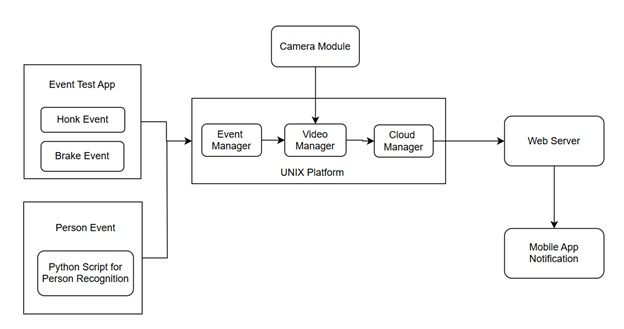
\includegraphics[width=1\linewidth]{System architecture.jpg}
    \caption{System Architecture}
  \label{fig:system-architecture}
\end{figure}
\subsection{Event Sources and Triggers}
There are two primary sources of events in the system:
\begin{itemize}
  \item \underline{Event Test App:}A simulation tool developed for triggering artificial events such as honk and brake events. This was essential during development and testing, allowing deterministic input and verification of system behaviour.
  \item \underline{Person Event Detection:}Implemented as a Python script using OpenCV, this module performs real-time person detection using live video feed or frames captured from the camera. Upon detecting a suspicious presence, it generates a person event and sends it to the Event Manager.
  \end{itemize}
These inputs represent external triggers that cause the system to begin recording and initiate further downstream operations.
\subsection{UNIX Platform and Modular Core}
The core components of the system are executed on a UNIX platform. These include the event manager, video manager, and cloud manager modules.
\begin{itemize}
    \item  \underline{Event Manager:} This is the central controller that receives input from both the event test app and the person detection script. It acts as the gateway to initiate the surveillance sequence. Upon receiving an event signal, it sends a control message to the video manager to begin processing and recording.
\end{itemize}

%•\underline{Video Manager:} Upon receiving the trigger signal,the video manager performs the core video recording operation.It uses a circular buffer to continuously store the last 30 seconds of video data from the Camera Module,ensuring preevent footage is available. When activated, it extracts both the 30 seconds before the event and 30 seconds after,encodes it using GStreamer,and writes the footage into an MP4 file.This ensures comprehensive event capture with context.\\
%• \underline{Cloud Manager:} Once the MP4 file is created, the video manager passes control to the cloud manager. This module handles the task of uploading the recorded file to a web server, along with the required metadata (e.g., event type, timestamp). The upload is done via HTTP POST requests to PHP based APIs hosted on an Apache server.
\subsection{Cloud Backend}
The Web Server is implemented using a local Apache installation, with PHP used to create REST APIs. These APIs handle:
\begin{itemize}

 \item  File reception and storage,
 \item  Metadata insertion into a MySQL database,
 \item  Notification triggers for newly uploaded files.   
\end{itemize}
The web server acts as the central repository for all video files and associated event data.\\
\underline{Mobile App and Notification System}:\\
Once the file is uploaded, the backend triggers a notification to the Mobile App. The app is designed to:
\begin{itemize}
\item  Receive push notifications when a new event is uploaded,
\item  Fetch the list of available videos using the API,
\item  Allow users to play selected videos directly from the server.
\end{itemize}
This provides realtime access to surveillance events from a remote device, completing the end to end system flow from detection to user alert.

% Additional project documentation artifacts
\chapter{Software Requirements Definition (SRD)}
\section{Purpose}
The Software Requirements Definition (SRD) describes the business context, stakeholder goals, and product boundary for the Intelligent Incident Surveillance Response System. The system is intended to provide event-based surveillance for vehicles by capturing relevant evidence, uploading it to a backend, and making it available through a mobile interface.

\section{Scope}
The product scope includes:
\begin{itemize}
\item Event generation from simulated and vision-based sources.
\item Event orchestration and recording control.
\item Buffered video recording with pre-event and post-event context.
\item Upload of event clips and metadata to cloud/backend services.
\item User notification and remote playback support through a mobile app.
\end{itemize}

The following are outside the current scope:
\begin{itemize}
\item Fleet-level analytics dashboards.
\item Automated legal workflow for claims processing.
\item Multi-vehicle live map tracking in production cloud.
\end{itemize}

\section{Stakeholders}
\begin{itemize}
\item Vehicle Owner: receives alerts and reviews incident evidence.
\item Fleet Operator: monitors incident clips across assigned vehicles.
\item Developer/Maintainer: configures trigger logic and backend services.
\item System Administrator: maintains database, upload APIs, and storage.
\end{itemize}

\section{Business and User Needs}
\begin{itemize}
\item Reduce unnecessary continuous recording and storage overhead.
\item Preserve contextual evidence before and after incidents.
\item Improve response time with near-real-time mobile notifications.
\item Provide simple remote review workflow for uploaded incidents.
\item Keep architecture modular for easy maintenance and upgrades.
\end{itemize}

\section{Assumptions and Constraints}
\begin{itemize}
\item Camera feeds are available with acceptable quality for trigger processing.
\item Local network and backend services are reachable during upload.
\item Platform components run in a UNIX/Linux environment.
\item Integration uses named pipes and API endpoints already defined in the project.
\item Security hardening is baseline and can be extended in future revisions.
\end{itemize}

\section{Success Criteria}
The SRD is considered satisfied when the system can detect a supported event, generate and store a complete incident clip (with pre/post context), upload it with metadata, and make it discoverable from the mobile interface with user notification.
\chapter{Software Requirements Specification (SRS)}
\section{Introduction}
This SRS defines functional and non-functional requirements for the Intelligent Incident Surveillance Response System implementation documented in this project.

\section{Functional Requirements}
\begin{longtable}{|p{1.6cm}|p{5.0cm}|p{7.6cm}|}
\hline
\textbf{ID} & \textbf{Requirement} & \textbf{Description} \\
\hline
FR-01 & Event Detection & The system shall detect supported trigger events from simulation input and computer-vision input. \\
\hline
FR-02 & Event Routing & The event manager shall validate events and dispatch recording commands to the recording subsystem. \\
\hline
FR-03 & Pre-event Buffer & The video manager shall preserve at least 30 seconds of pre-event video context in memory. \\
\hline
FR-04 & Post-event Capture & The system shall capture at least 30 seconds of post-event footage after a valid trigger. \\
\hline
FR-05 & Clip Generation & The system shall generate a playable MP4 incident clip combining pre-event and post-event segments. \\
\hline
FR-06 & Metadata Storage & The backend shall store clip metadata including timestamp, event type, and storage path. \\
\hline
FR-07 & Cloud Upload & The cloud manager shall upload the generated clip to server storage over HTTP API. \\
\hline
FR-08 & Notification & The mobile client shall receive event notifications after successful backend update. \\
\hline
FR-09 & Incident Listing & The mobile client shall retrieve and display available incident recordings. \\
\hline
FR-10 & Playback & The mobile client shall play selected recordings from backend-hosted media. \\
\hline
\end{longtable}

\section{Non-Functional Requirements}
\begin{itemize}
\item NFR-01 Performance: End-to-end flow from event to clip availability should complete within operationally acceptable delay for local deployment.
\item NFR-02 Reliability: Module failures should be logged with enough detail for diagnosis and recovery.
\item NFR-03 Maintainability: Components shall remain modular and independently testable.
\item NFR-04 Compatibility: Generated clips shall be playable on common Android media stacks.
\item NFR-05 Security: Upload and API access shall enforce authentication controls and secure transport where available.
\item NFR-06 Scalability: Backend schema and API design shall support growth in incident volume.
\end{itemize}

\section{External Interface Requirements}
\subsection{Software Interfaces}
\begin{itemize}
\item Python modules for event processing and orchestration.
\item Backend APIs implemented with Apache/PHP and MySQL.
\item Firebase-based notification pathway for mobile alerting.
\end{itemize}

\subsection{Communication Interfaces}
\begin{itemize}
\item Named pipes for internal module signaling.
\item HTTP endpoints for file upload and incident metadata operations.
\end{itemize}

\section{Traceability Summary}
\begin{itemize}
\item FR-01/FR-02 map to event modules.
\item FR-03/FR-04/FR-05 map to recording service and encoding pipeline.
\item FR-06/FR-07 map to backend upload and database handling.
\item FR-08/FR-09/FR-10 map to mobile and notification integration.
\end{itemize}
\chapter{Unit Testing (UT)}
\section{Objective}
The unit-testing objective is to verify correctness of module-level logic before full integration. The focus is on deterministic event handling, recording boundaries, metadata consistency, and API response behavior.

\section{Unit Test Scope}
\begin{itemize}
\item Event parsing and classification logic.
\item Trigger-to-record command dispatch.
\item Buffer window assembly (pre-event and post-event).
\item Upload request creation and retry behavior.
\item Metadata generation and persistence mapping.
\end{itemize}

\section{Test Environment}
\begin{itemize}
\item Development host running the project Python modules.
\item Local backend services (Apache, PHP, MySQL).
\item Controlled test inputs (simulated honk/brake/person events).
\end{itemize}

\section{Representative Unit Test Cases}
\begin{longtable}{|p{1.7cm}|p{4.0cm}|p{4.2cm}|p{4.3cm}|}
\hline
\textbf{Test ID} & \textbf{Target Unit} & \textbf{Input/Condition} & \textbf{Expected Result} \\
\hline
UT-01 & Event parser & Valid event payload & Event type resolved and routed without error \\
\hline
UT-02 & Event parser & Invalid/malformed payload & Rejected safely; diagnostic log written \\
\hline
UT-03 & Recording window logic & Trigger at time $t$ & Clip contains buffer before $t$ and capture after $t$ \\
\hline
UT-04 & Upload client & Backend reachable & HTTP success and metadata update acknowledged \\
\hline
UT-05 & Upload client & Backend timeout/failure & Retry policy executed and failure status logged \\
\hline
UT-06 & Metadata mapper & New incident clip data & Correct DB/API payload fields populated \\
\hline
\end{longtable}

\section{Pass Criteria}
\begin{itemize}
\item All critical unit tests pass for event routing and clip generation.
\item Failure paths return controlled errors and emit actionable logs.
\item Metadata fields used by the mobile application are complete and valid.
\end{itemize}

\section{Risk-Based Notes}
\begin{itemize}
\item Timing-sensitive tests can show variance depending on host load.
\item Camera source interruptions should be tested separately under fault-injection scenarios.
\item Notification timing validation is verified primarily in integration testing.
\end{itemize}
\chapter{High-Level Design (HLD)}
\section{Architecture Overview}
The system follows a modular event-driven architecture. Each subsystem is isolated by responsibility and communicates through defined interfaces to reduce coupling and improve maintainability.

\section{Major Subsystems}
\begin{itemize}
\item Event Source Layer: generates events from simulation and vision detection.
\item Orchestration Layer: validates events and triggers recording workflow.
\item Recording Layer: builds incident clips from buffered and live frames.
\item Cloud Layer: uploads clips and stores incident metadata.
\item Client Layer: displays incidents and receives notifications.
\end{itemize}

\section{Component Responsibilities}
\begin{longtable}{|p{3.2cm}|p{3.0cm}|p{7.8cm}|}
\hline
\textbf{Component} & \textbf{Primary File/Module} & \textbf{Responsibility} \\
\hline
Event Producer & data\_monitor.py / debug\_update.py & Emit controlled trigger events for test and validation flows. \\
\hline
Event Controller & EventManager.py & Receive and coordinate trigger handling across downstream modules. \\
\hline
Recording Service & recording\_service.py & Manage incident clip creation and recording state transitions. \\
\hline
Cloud/Firebase Adapter & firebase\_manager.py & Push notifications and cloud-facing update operations. \\
\hline
Operator UI & main\_gui.py & Provide local control and status visibility for operators. \\
\hline
Utility Layer & utils.py & Shared helper functions used across modules. \\
\hline
\end{longtable}

\section{Data Flow Summary}
\begin{enumerate}
\item Event source emits trigger.
\item Event controller validates trigger and initiates recording action.
\item Recording service assembles incident clip with contextual buffer.
\item Cloud adapter uploads clip metadata and notifies clients.
\item Client views updated incident list and plays selected clips.
\end{enumerate}

\section{Design Constraints}
\begin{itemize}
\item Timely event processing with low overhead on local hardware.
\item Predictable inter-module interfaces for easier debugging.
\item Compatibility with local backend deployment stack.
\end{itemize}

\section{Design Rationale}
This architecture prioritizes clarity and fault isolation. If one service degrades, logs and boundaries make diagnosis straightforward while preserving the ability to upgrade modules incrementally.
\chapter{UML Diagram}
\section{Use Case Diagram (Textual)}
% \begin{framed}
\begin{figure}[H]
    \centering
    
\includegraphics[width=0.5\linewidth]{Report//figures/UseCase.png}
    \caption{Use Case Diagram}
  \label{fig:system-architecture}
\end{figure}
% \end{framed}
\newpage


\section{Class Diagram (Conceptual)}

\begin{figure}[H] % <-- Added [H] right here to force exact placement
    \centering
    
\includegraphics[width=0.8\linewidth]{Report//figures/ClassDiagram.png}
    \caption{Class Diagram}
    \label{fig:system-architecture}
\end{figure}

\newpage

\section{Sequence Diagram (Event to Notification)}
\begin{figure}[H]
    \centering
    
\includegraphics[width=1\linewidth]{Report//figures/sequenceDiagram.png}
    \caption{Sequence Diagram}
    \label{fig:placeholder}
\end{figure}

\section{Deployment Diagram (Logical Nodes)}
\begin{figure}[H]
    \centering
    
\includegraphics[width=0.8\linewidth]{Report//figures/DeploymentDiagram.png}
    \caption{Deployement Diagram}
    \label{fig:placeholder}
\end{figure}

\chapter{User Guide}
\section{Purpose}
This guide explains how to run the Intelligent Incident Surveillance Response System in a local development setup and how to verify end-to-end behavior.

\section{Prerequisites}
\begin{itemize}
\item Python environment with project dependencies.
\item Backend services configured (Apache, PHP, MySQL).
\item Firebase credentials configured for notification features.
\item Camera/video input source available for event simulation or detection.
\end{itemize}

\section{Project Files of Interest}
\begin{itemize}
\item main\_gui.py: local control interface.
\item EventManager.py: event coordination logic.
\item recording\_service.py: clip generation logic.
\item firebase\_manager.py: cloud/notification integration.
\item data\_monitor.py, debug\_update.py, debug\_firebase\_test.py: testing and debug helpers.
\end{itemize}

\section{Startup Procedure}
\begin{enumerate}
\item Start backend services and verify database connectivity.
\item Confirm configuration files and credentials are present.
\item Launch monitoring and orchestration modules.
\item Launch the local GUI if interactive operation is required.
\item Trigger a test event and verify clip creation and upload.
\end{enumerate}

\section{Operational Workflow}
\begin{enumerate}
\item System waits in monitoring state.
\item Trigger event occurs (simulated or vision-based).
\item Recording module builds incident clip with context.
\item Clip metadata is stored and notification is sent.
\item User opens client app and reviews incident list/playback.
\end{enumerate}

\section{Troubleshooting}
\begin{itemize}
\item No notification received: check Firebase key path and backend notification logs.
\item Clip missing: verify recording service status and available disk space.
\item Upload failure: verify API endpoint reachability and backend permissions.
\item Empty incident list: confirm metadata insertion in database tables.
\end{itemize}

\section{Best Practices}
\begin{itemize}
\item Keep system clock synchronized across modules.
\item Use controlled event simulations before live camera testing.
\item Archive old clips periodically to maintain storage performance.
\item Review logs after each test cycle to catch intermittent issues.
\end{itemize}

\chapter{Module Description}
The system was divided into five functional modules so that acquisition, decision-making, storage, and user interaction could be developed and tested independently. The modular design also simplified debugging and made it possible to replace or improve individual components without affecting the entire system.

\section{Event App}
The event app is responsible for generating trigger events for the surveillance pipeline. It supports both simulated events, such as honking or sudden braking, and computer-vision-based detection of suspicious human presence near the vehicle. The module was implemented in Python and used OpenCV for frame capture and preprocessing, while MediaPipe was used to strengthen human detection in live video streams. Whenever a valid event is detected, the module forwards an event message to the event manager through a named pipe.

\section{Event Manager}
The event manager acts as the central coordinator of the system. It receives event messages from the event app, validates the incoming trigger, and instructs the video manager to preserve the corresponding surveillance clip. This module was implemented in C++ to provide deterministic control and efficient inter-process communication. By separating event coordination from event generation, the system maintains clear control flow and supports future expansion to additional trigger sources.

\section{Video Manager}
The video manager performs the core recording task. It continuously maintains a circular buffer containing the most recent 30 seconds of video so that important context before a trigger event is not lost. Once an event is received, the module stores the buffered pre-event segment together with 30 seconds of post-event footage, producing a 60-second incident clip. GStreamer was used for encoding, muxing, and writing the final MP4 file, ensuring playback compatibility and efficient handling of the incoming video stream.

\section{Cloud Manager}
The cloud manager transfers the recorded video clip to the backend server and stores the associated metadata. The backend was implemented using Apache, PHP, and MySQL. On receiving a completed clip from the video manager, the cloud manager uploads the file through HTTP-based APIs and records relevant information such as file name, timestamp, and event type. This module enables remote access to the captured footage and serves as the bridge between the embedded platform and the mobile application.

\section{Mobile Application}
The Android application provides the user-facing interface of the system. It displays the list of uploaded recordings, supports playback of selected incident videos, and receives notifications whenever a new event is uploaded. This allows the vehicle owner to remain informed even when away from the vehicle. The mobile application therefore completes the end-to-end workflow by converting backend updates into immediate and usable information for the user.
%7.\underline{\textbf{End to End Workflow Integration}}\\
%To integrate all modules into a working pipeline from event detection to video recording, cloud upload, and mobile notification providing a fully automated surveillance system.
\chapter{Implementation}
The Smart Vehicle Surveillance System was developed using multiple programming languages, tools, and platforms. Its modular design allowed parallel development, isolated testing, and focused optimization of individual modules, reducing complexity and facilitating debugging.\par
The system was implemented on a UNIX based Linux environment, which supports multi-process operations, inter process communication, and real-time data processing. Modules communicated through UNIX named pipes (FIFOs), enabling efficient one way streams between producer-consumer components.
\section{Event Detection (event app)}
\begin{itemize}

    \item 
Implemented in Python.
    \item 
 Simulated events (e.g., braking and honking) and real-world detection of suspicious individuals using OpenCV and MediaPipe.
    \item 
 Human detection leveraged OpenCV for frame processing and MediaPipe models to identify persons within the camera frame.
    \item 
 Detected events were sent to the Event Manager through a named pipe.
 \end{itemize}
\section{Event Manager (event manager)}
\begin{itemize}
 \item  Developed in C++.
 \item  Served as the central controller, interpreting events from the              event app.
 \item  Triggered the Video Manager to start recording when an event was            confirmed.
 \end{itemize}
\section{Video Manager (video manager)}
\begin{itemize}
  

  \item  Implemented in C++ using the GStreamer multimedia framework.
  \item  Maintained a 30 second circular buffer of pre event frames.
  \item  Upon trigger, combined pre event and 30 second post event video into a      single MP4 file.
  \item  GStreamer handled encoding, muxing, and buffering, ensuring reliable        timing and video quality.
\end{itemize}
\section{Cloud Manager (cloud manager)}
\begin{itemize}
  \item  Managed the upload of MP4 files to a locally hosted Apache server.
  \item PHP scripts handled file reception via HTTP POST and stored metadata in a   MySQL database.
  \item Used libcurl for reliable uploads and implemented retry mechanisms for      network failures.
  \end{itemize}
\section{Mobile App (Android)}
\begin{itemize}
  \item Developed in Java for Android devices.
  \item Connected to the backend to fetch and display uploaded videos.
 \item Supported video playback using the native Android media player.
  \item Received real-time push notifications via Firebase Cloud Messaging (FCM)    whenever a new video was uploaded.
  \end{itemize}
\section{Development Approach}
\begin{itemize}
 
   \item Early prototypes of each module were developed to test feasibility,         library behavior, and system responsiveness.
   \item  Iterative refinements were performed within modules despite following the    Waterfall model, such as optimizing the circular queue for memory usage     and frame timing.
  \item Functional and integration testing ensured all modules worked together      reliably.
  \end{itemize}
\section{Deployment}
\begin{itemize}
    \item 
The system is fully implemented, integrated, and tested in a local           environment, including the Apache server, database, and connected           cameras.
    \item 
 The Android app has been tested on physical devices for playback and        notifications.
    \item 
 Deployment scripts automate service startup, network configuration, and     headless operation on embedded UNIX platforms.
 \end{itemize}
\begin{figure}[h]
    \centering
    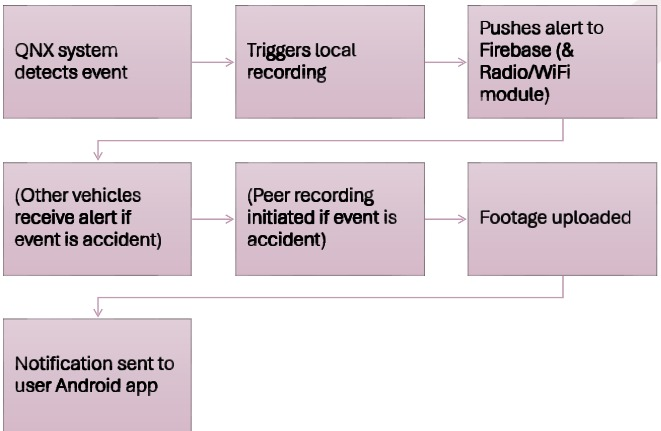
\includegraphics[width=1\linewidth]{Flow Fiagram.jpg}
  \caption{System Flow Diagram}
    \label{fig:system-flow}
\end{figure}
\chapter{Result}
The integrated prototype was functionally validated in a controlled local environment using simulated trigger events and computer-vision-based person detection. The evaluation focused on confirming the end-to-end behaviour of the system rather than establishing benchmark-level quantitative accuracy. The following outcomes were consistently observed during testing:\\

\begin{itemize}
  \item Trigger events generated by the event app were correctly received by the event manager.
  \item The video manager preserved buffered pre-event footage and produced a complete incident clip with post-event context.
  \item Recorded clips were uploaded successfully to the local server along with the associated metadata.
  \item The Android application was able to list uploaded videos, play the selected recording, and receive event notifications after upload.
\end{itemize}

These results show that the proposed architecture is suitable for event-driven surveillance and remote incident review. The prototype demonstrated that selective recording can capture relevant evidence while reducing the storage overhead associated with continuous dash-camera operation. The screenshots presented in this chapter illustrate the person-detection stage and the mobile application interface used for remote access to recorded clips.

\begin{figure}[h]
    \centering
    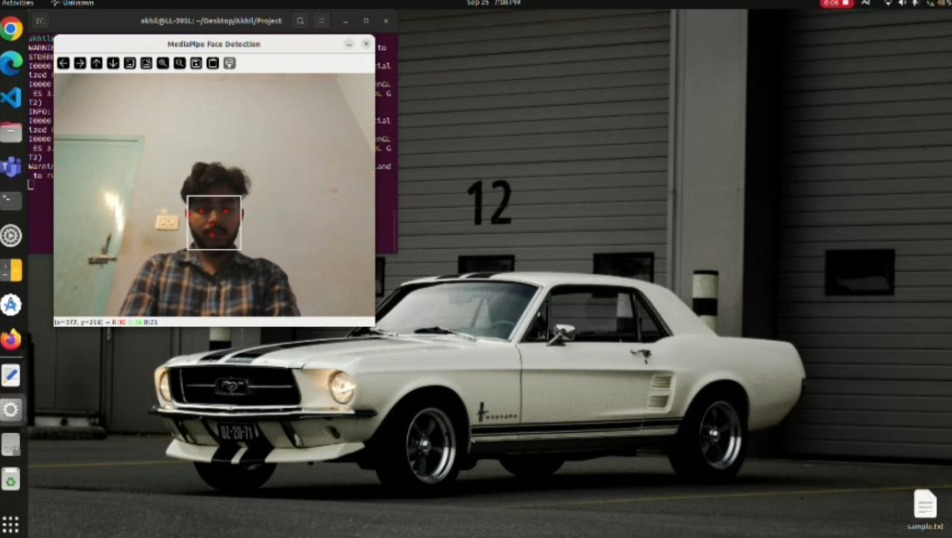
\includegraphics[width=1\linewidth]{person detection.jpg}
    \caption{Person Detection}
  \label{fig:person-detection}
\end{figure}
\begin{figure}
    \centering
    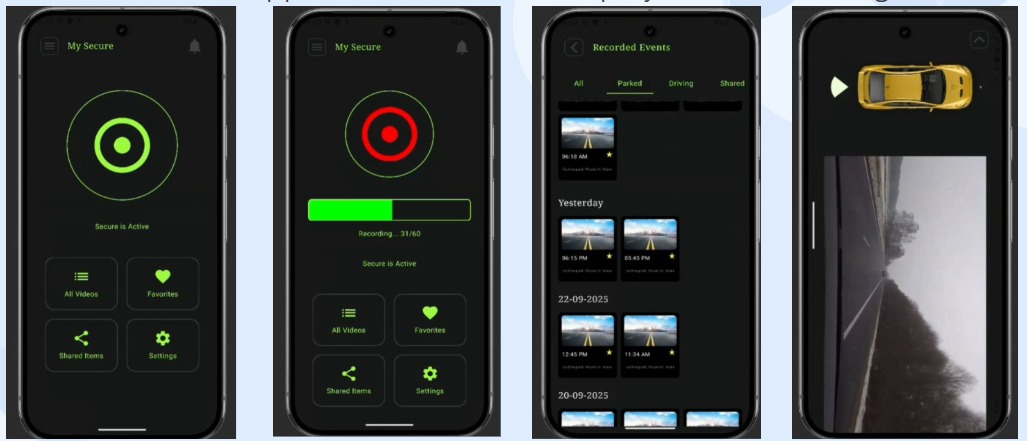
\includegraphics[width=1\linewidth]{mobile app.jpg}
    \caption{Mobile App}
  \label{fig:mobile-app}
\end{figure}
\par
Although the functional objectives were achieved, formal quantitative evaluation remains a scope for future work. Metrics such as event-detection precision, false-positive rate, recording latency, cloud upload delay, and notification latency should be measured systematically in a larger test campaign before real-world deployment.
\chapter{Conclusion}
This project successfully demonstrated a modular and event-driven vehicle surveillance system capable of detecting relevant events, recording buffered video clips, uploading them to a cloud backend, and notifying the user through a mobile application. By combining OpenCV- and MediaPipe-based event detection with GStreamer-based video processing and a lightweight web backend, the system moved beyond passive recording and provided a more responsive security workflow.

The use of independent processes connected through named pipes improved modularity and simplified system integration. The video manager preserved 30 seconds of pre-event footage and combined it with 30 seconds of post-event footage, thereby producing incident clips with meaningful context. The cloud manager and Android application further extended the usefulness of the system by making recorded events accessible remotely.

The work also highlighted practical limitations. Person detection accuracy can still be improved under challenging lighting and environmental conditions, and the system has not yet undergone large-scale quantitative benchmarking. In addition, further hardening is required in areas such as fault tolerance, network resilience, and secure deployment.

Future work may focus on improving detection robustness, measuring system latency under varied operating conditions, extending the trigger set to additional vehicle events, and migrating from a local backend to a production-ready secure cloud platform. Even in its current form, the prototype demonstrates the technical feasibility and practical value of intelligent, event-based vehicle surveillance.
\chapter{References}
\begin{thebibliography}{99}

\bibitem{patel2024}
M. Patel, A. Shah, and R. Kumar, ``Proposed method for car theft prevention techniques,'' \textit{International Journal of Technology Research and Studies}, vol. 12, no. 3, pp. 45--59, 2024.

\bibitem{rocky2024}
A. Rocky, Q. J. Wu, and W. Zhang, ``Review of accident detection methods using dashcam videos,'' \textit{IEEE Transactions on Intelligent Transportation Systems}, vol. 25, no. 8, pp. 8356--8367, 2024.

\bibitem{rehman2018}
M. T. Rehman, N. Khan, and S. Ali Shah, ``Live view car surveillance system,'' \textit{IEEE Access}, vol. 6, pp. 29488--29496, 2018.

\bibitem{tesla2023}
Tesla, Inc., ``Sentry Mode: Guarding your Tesla,'' 2023. Available: \url{https://www.tesla.com/blog/sentry-mode-guarding-your-tesla}

\bibitem{cosens2023}
A. Arev, J. Park, A. Sheikh, \textit{et al.}, ``COSENS: Collaborative and opportunistic sensing of road events by vehicles' cameras,'' 2023.

\bibitem{park2022}
J. Park and S. Lee, ``Cloud-assisted event detection in vehicular networks,'' 2022.

\bibitem{ahmad2022}
I. Ahmad and M. A. Khan, ``Real-time data streaming in connected vehicles,'' \textit{Journal of Computer Networks and Communications}, 2022, pp. 1--11.

\end{thebibliography}
\end{document}